\chapter{\leavevmode \newline Methods}
\label{chap:Methods}

Exploration on granular planetary terrain is a task marked by uncertainty, variability, and risk. Unlike rigid or structured environments where surface characteristics are relatively predictable, granular media such as regolith can shift suddenly under pressure. These shifts often occur without any visual cues. A successful navigation algorithm must not only plan paths toward a goal but must also adapt its behavior in real time based on what the robot learns through physical interaction.

This chapter presents the complete method developed to address these challenges. The system combines safe Bayesian global planning with geometry-based local control. The fundamental idea is that a legged robot, through proprioceptive interaction, can actively map the terrain's mechanical properties, update its internal risk estimates, and select both where to go and how to get there, while maintaining operational safety and supporting scientific objectives.

\section{Terrain-Aware Navigation as a Sequential Decision Problem}

Legged robots are uniquely suited to granular terrain because their limbs can serve two functions: enabling mobility and acting as embedded sensors. Each step provides an opportunity for measurement and becomes an input to an evolving internal model of terrain risk.

Navigation in this context can be treated as a sequential decision-making process under uncertainty. The robot must choose its next move based on local terrain observations, estimated risks, and proximity to the goal, while ensuring that all movement adheres to strict safety constraints. This challenge is met by combining two core components:

\begin{enumerate}
    \item A probabilistic planner that incrementally expands a certified safe set of traversable terrain using terrain observations and confidence-based reasoning.
    \item A reactive controller based on diffeomorphic transformation that enables real-time, geometry-aware path execution within certified safe regions.
\end{enumerate}

\section{Problem Statement}
\label{sec:Problem_Formulation}

The robot operates within a two-dimensional discretized domain \( D \subset \mathbb{R}^2 \), where each point has an unknown terrain property, such as shear strength or cohesion, that influences traversability. The objective is to move from an initial location \( x_0 \) to a goal location \( x_g \), ensuring that all intermediate positions lie within regions classified as safely traversable.

We define \( f(x) \) as a scalar-valued function representing the traversability of terrain at location \( x \), where higher values correspond to more easily traversable regions. This function is treated abstractly and may encode various underlying physical or empirical terrain characteristics depending on the application context. A fixed threshold \( h \) is used to determine safety: terrain is considered safe if \( f(x) \geq h \), and unsafe if \( f(x) < h \). The values of \( f(x) \) and \( h \) are not assumed to carry physical units or universal semantics; rather, they serve as internally consistent constructs for distinguishing safe and unsafe terrain within the chosen representation framework.


Key assumptions and constraints are as follows:
\begin{itemize}
    \item Terrain risk is a continuous but unknown function over space.
    \item Proprioceptive terrain measurements are available only at the robot’s current location.
    \item Navigation must maintain high-confidence safety guarantees at all times.
\end{itemize}

\section{Confidence-Guided Terrain Expansion}
\label{sec:ConfidenceGuided}

The planner maintains a probabilistic model of terrain risk using a Gaussian Process (GP). At each step, it updates terrain predictions and refines a subset of the environment certified as safe.

This method draws inspiration from prior work on safe exploration algorithms such as SafeOPT and SafeUCB \cite{safeopt, losalka2023msafeucb}, but differs in structure and execution. In particular, the focus of this work is not on maximizing a reward function, but on expanding reachable terrain while ensuring probabilistic safety at every decision point.

\subsection{Gaussian Process Terrain Modeling}

The robot uses proprioceptive data to train a Gaussian Process (GP) model over \( D \), producing a mean prediction \( \mu_t(x) \) and standard deviation \( \sigma_t(x) \) at each location \( x \in D \). The GP uses a radial basis function (RBF) kernel:
\[
k(x, x') = \sigma^2 \exp\left(-\frac{\|x - x'\|^2}{2 \ell^2}\right)
\]
where \( \sigma^2 \) is the kernel variance and \( \ell \) is the lengthscale, both selected manually based on the expected variability of the proprioceptive signal. These hyperparameters are fixed at deployment time.

The model is updated recursively using all past measurements for computational efficiency. At each step, the robot collects a new proprioceptive terrain measurement \( y_t \) at position \( x_t \), then incorporates this into the GP model to update posterior predictions across the domain.

\subsection{Safe Set Expansion}

A fixed exploration parameter \( \beta_t \) is used to control the width of confidence intervals:
\begin{equation}
Q_t(x) = \left[\mu_{t-1}(x) \pm \sqrt{\beta_t}\, \sigma_{t-1}(x)\right]
\end{equation}
This formulation is adapted from the SafeOPT algorithm introduced by \textcite{safeopt}, where confidence intervals are used to balance safety with informative sampling. The value of \( \beta_t \) should be chosen via empirical tuning to balance conservative exploration with steady progress.

The resulting confidence bounds are intersected with prior confidence sets to form updated constraints:
\begin{equation}
    C_t(x) = C_{t-1}(x) \cap Q_{t-1}(x)
\end{equation}
From these sets, the lower and upper bounds are defined as:
\begin{equation}
    \ell_t(x) = \min C_t(x), \quad u_t(x) = \max C_t(x)
\end{equation}
and the interval width is computed as:
\begin{equation}
    w_t(x) = u_t(x) - \ell_t(x)
\end{equation}

\begin{algorithm}[H]
\caption{Safe Optimization for 2D Navigation}
\begin{algorithmic}[1]
\Require Sample set \( D \), GP prior \( (\mu_0, k, \sigma_0) \), Lipschitz constant \( L \), seed set \( S_0 \), safety threshold \( h \), goal location \( x_g \), number of expanders to consider \( n \)
\State \( C_0(x) \gets [h, \infty), \, \forall x \in S_0 \)
\State \( C_0(x) \gets \mathbb{R}, \, \forall x \in D \setminus S_0 \)
\State \( Q_0(x) \gets \mathbb{R}, \, \forall x \in D \)
\For{each time step \( t = 1, 2, \ldots \)}
    \State \( C_t(x) \gets C_{t-1}(x) \cap Q_{t-1}(x) \)
    \State \( S_t \gets \bigcup_{x \in S_{t-1}} \left\{ x' \in D \,\middle|\, \ell_t(x) - L \|x-x'\| \geq h \right\} \)
    \State \( G_t \gets \left\{ x \in S_t \,\middle|\, g_t(x) > 0 \right\} \)
    \State Sort \( G_t \) by \( \|x - x_g\| \) in ascending order
    \State Let \( G_t^{(n)} \subseteq G_t \) be the top \( n \) nearest expanders
    \State \( x_t \gets \arg\max_{x \in G_t^{(n)}} w_t(x) \)
    \State Observe \( y_t = f(x_t) + n_t \)
    \State Compute \( Q_t(x) \) for all \( x \in S_t \)
\EndFor
\end{algorithmic}
\end{algorithm}

To identify \(G_t\), the function
\begin{equation}
    g_t(x) = \left| \left\{ x' \in D \setminus S_t \,\middle|\, u_t(x) - L \|x - x'\| \geq h \right\} \right|
\end{equation}

is defined, evaluating the expansion potential of each point.

This strategy combines uncertainty-driven sampling with spatial prioritization to ensure that each move both refines the terrain model and progresses toward the mission objective.

The robot selects the next point to sample by balancing two objectives:
\begin{itemize}
    \item Reducing model uncertainty (exploration)
    \item Making progress toward the mission goal (exploitation)
\end{itemize}

After constructing the safe set \( S_t \) and identifying the candidate expanders \( G_t \subseteq S_t \), the robot must select the next point at which to sample terrain. Rather than choosing purely based on uncertainty or purely based on proximity to the goal, \algoname{} employs a hybrid strategy to guide exploration in a goal-directed yet uncertainty-aware manner.

\subsubsection{Next Parameter Selection}

The new selection procedure is as follows:
\begin{enumerate}
    \item For each point \( x \in G_t \), compute its distance to the goal \( \|x - x_g\| \).
    \item Sort all points in \( G_t \) in ascending order of distance to the goal.
    \item Consider only the top \( n \) nearest expanders, where \( n \) is a configurable parameter.
    \item Among these \( n \) expanders, select the point with the largest confidence interval width \( w_t(x) \).
\end{enumerate}

This approach prioritizes expanders that are spatially aligned with the mission objective while still favoring those that offer informative terrain data. It mitigates the risk of wasting samples on irrelevant or backward directions and prevents purely greedy selection based on proximity alone, which might lead into regions of high uncertainty without expanding the safe set.

By focusing on a small subset of candidate expanders that are both near the goal and informative, the planner ensures steady, efficient progress toward the goal while incrementally enlarging the verified safe zone.

\section{Reactive Voronoi-Based Navigation}
\label{sec:VoronoiNavigation}

While the planner identifies the next point to move toward, executing safe and efficient motion between steps requires a robust local navigation strategy. Classical global planners, such as A* and RRT*, require full replanning after significant environmental updates, making them unsuitable for highly dynamic, partially known terrains.

Instead, a reactive control framework inspired by \textcite{vasilopoulos2021reactivenavigationpartiallyfamiliar} is implemented.

\subsection{Synthesizing Pseudo-Physical Obstacles}

To support reactive navigation, the robot must construct geometric representations of both safe and hazardous terrain regions from its evolving internal risk map. This process transforms pointwise risk predictions into polygonal approximations of safe space and its complement, enabling geometry-aware motion planning.

The environment is discretized into a two-dimensional grid. In simulation, this grid is aligned with the resolution of the ground truth map for consistency. In real-world deployments, however, the resolution becomes a tunable parameter. Higher resolutions enable more detailed boundary tracking but increase computational overhead, while lower resolutions reduce map fidelity in favor of speed and memory efficiency.

The conversion from safe points to obstacle geometry proceeds as follows:

\begin{enumerate}
    \item \textbf{Cluster Formation:} The current safe set \( S_t \) is partitioned into disjoint spatial clusters \( \{ S_{ti} \} \) using a combination of KD-tree nearest-neighbor queries and union-find data structures. Each cluster represents a contiguous region of confidently traversable terrain.

    \item \textbf{Concave Hull Construction:} For each cluster \( S_{ti} \), a concave hull \( H_{ti} \) is generated using the algorithm described by \textcite{park2013concavehull}, which takes as parameters a relative concavity level \( \mathcal{C} \) and a local threshold \( L_{th} \). These settings determine the hull’s shape resolution and computational complexity. In our implementation, we select high concavity values to tightly wrap each cluster. While these parameters influence geometric fidelity, they do not affect overall safety guarantees and may be tuned based on application requirements.

    \begin{figure}[h]
        \centering
        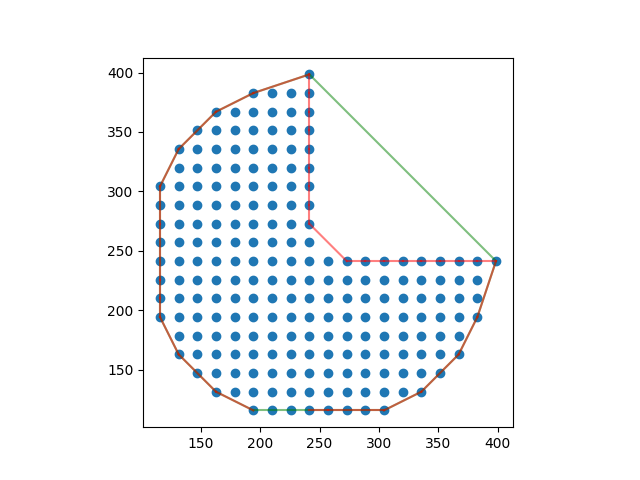
\includegraphics[width=0.7\linewidth]{figures/concave_hull_example.png}
        \caption{Visualization of a concave hull generated from point clusters. Image adapted from the \texttt{cubao/concave\_hull} GitHub repository \cite{cubao2024concavehull}. Licensed under the MIT License.}
        \label{fig:concave-hull}
    \end{figure}


    \item \textbf{Workspace Definition:} A bounding rectangle \( \mathcal{W}_e \) is formed to enclose all \( H_{ti} \) regions:
    \begin{equation}
    \mathcal{W}_e := \left\{ x \in \mathbb{R}^2 \,\middle|\, \min_i H_{ti}^{(1)} \leq x_1 \leq \max_i H_{ti}^{(1)},\; \min_i H_{ti}^{(2)} \leq x_2 \leq \max_i H_{ti}^{(2)} \right\}
    \end{equation}

    \begin{figure}[h]
        \centering
        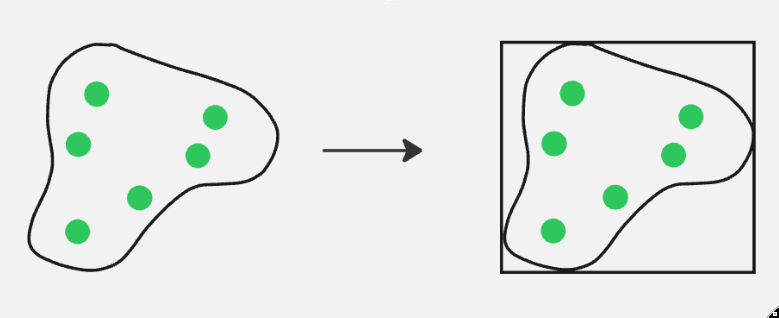
\includegraphics[width=0.7\linewidth]{figures/bounds.png}
        \caption{Visualization of bounding box creation. Green dots are fictional locations of safe samples, inner shape is depiction of safe area.}
        \label{fig:concave-hull}
    \end{figure}

    \item \textbf{Obstacle Extraction:} The regions not covered by the union of safe hulls are treated as pseudo-physical obstacles:
    \begin{equation}
    \mathcal{O}_t := \mathcal{W}_e \setminus \bigcup_{i} H_{ti}
    \end{equation}

    \item \textbf{Polygon Simplification:} The obstacle set \( \mathcal{O}_t \) is polygonal by construction but may contain excessive vertices. Each obstacle polygon is simplified using the Douglas-Peucker algorithm to reduce computational cost while preserving topology for subsequent triangulation and transformation.
\end{enumerate}

The resulting polygon set \( \mathcal{O}_t \) is used by the reactive controller to generate safe, smooth navigation commands around terrain hazards that have been inferred from contact-based measurements.

\subsection{Diffeomorphic Mapping and Reactive Control}

To enable real-time obstacle-aware motion without full replanning, we adopt a reactive navigation framework based on the approach proposed by \textcite{vasilopoulos2021reactivenavigationpartiallyfamiliar}. Their method provides a systematic means to guarantee obstacle avoidance and goal convergence in planar environments with polygonal obstacles, by leveraging a diffeomorphic transformation to map the physical space into a geometrically simplified model space.

We implement the core structure of their controller and adapt it to operate on pseudo-physical obstacles derived from proprioceptive terrain assessments. The application of this method in our context is novel, particularly in how the safe terrain regions are estimated and transformed dynamically based on risk-driven sampling.

Each polygon in the obstacle set \( \mathcal{O}_t \) is first triangulated using the Ear Clipping method \cite{ELGINDY1993719}. The resulting set of triangles is organized into a tree structure, where leaf triangles are recursively mapped onto their parents, and the root triangle is ultimately mapped onto a disk. This hierarchical transformation process defines a global diffeomorphism \( \mathbf{h}(x) \) from the original workspace to a simplified model space free of obstacles.

\begin{figure}[H]
    \centering
    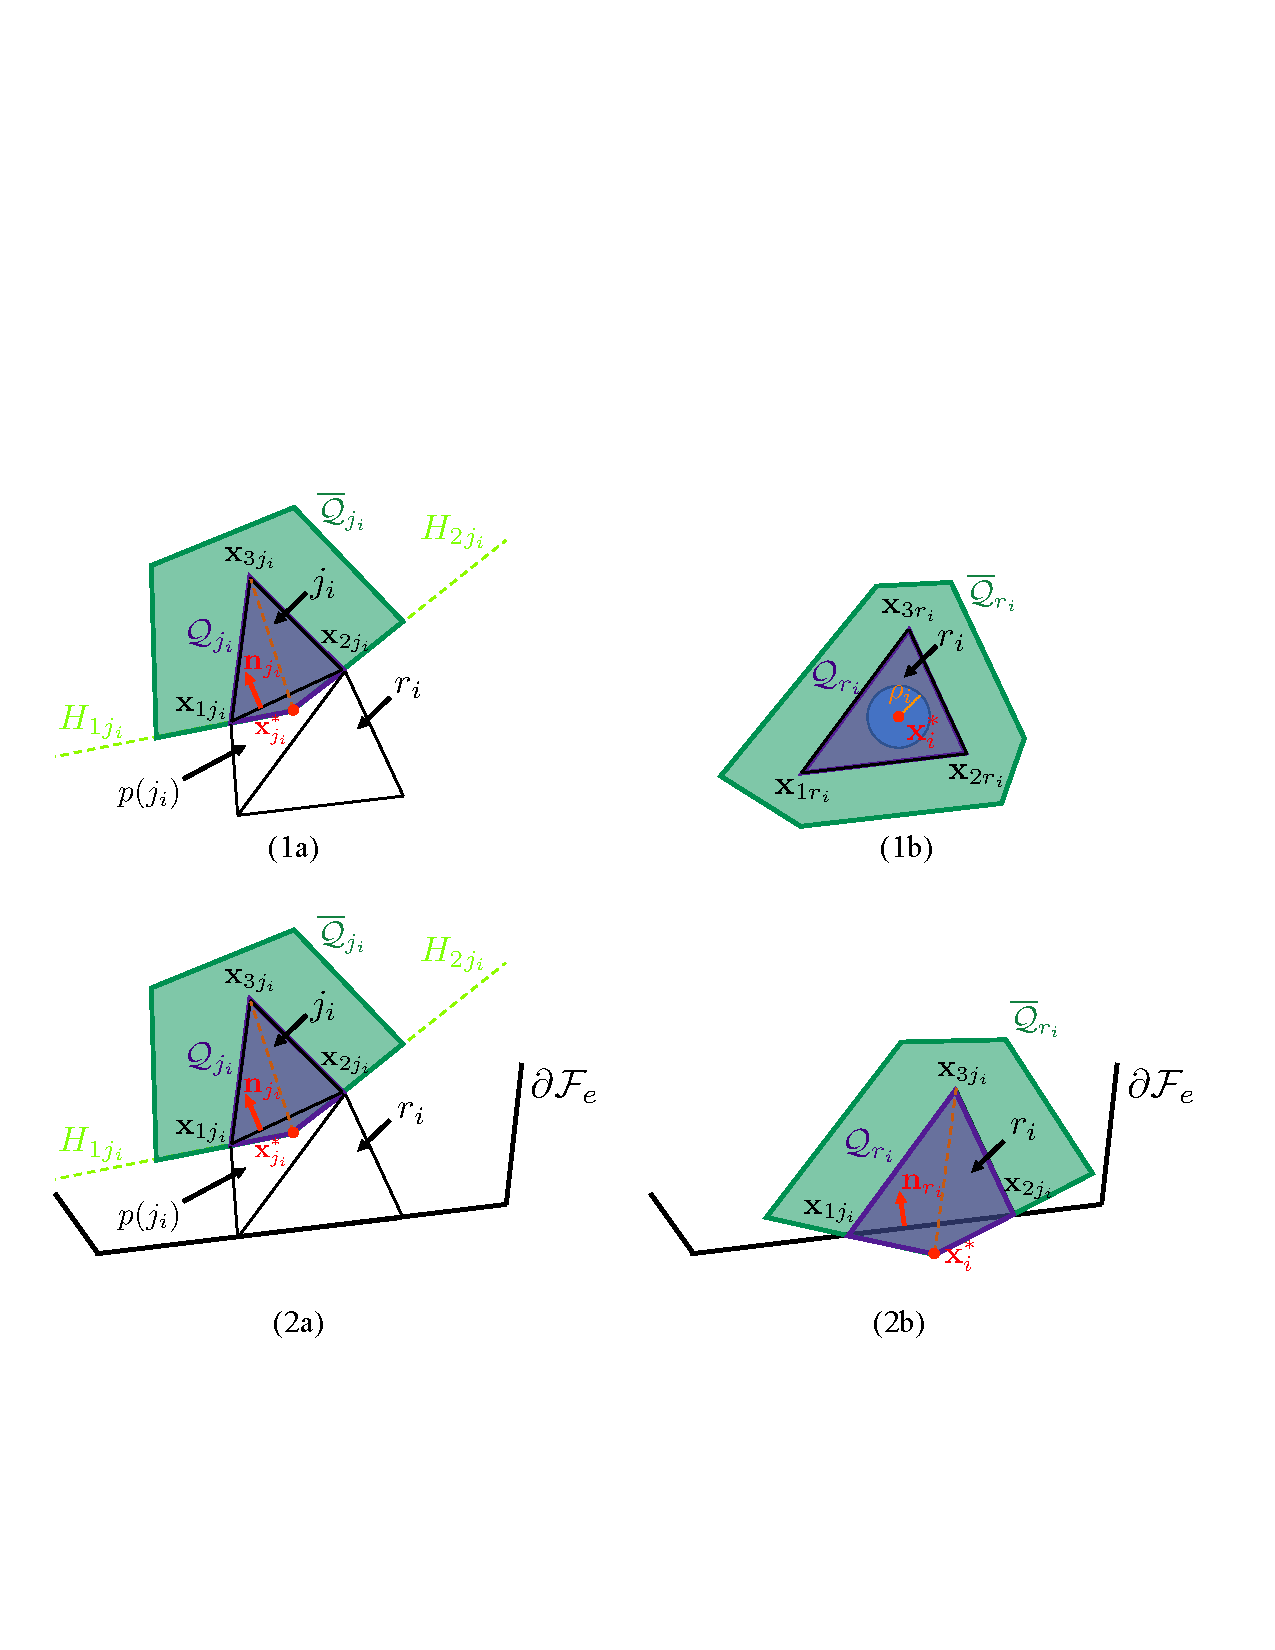
\includegraphics[width=0.8\linewidth]{figures/purging.pdf}
    \caption{Top row: (1a) A leaf triangle is mapped onto its parent triangle; (1b) A root triangle is mapped onto a disk centered at \( \mathbf{x}_i \) with radius \( \rho_i \). 
    Bottom row: (2a) A leaf triangle mapped onto its parent; (2b) A root triangle mapped onto the freespace border. 
    Figure reproduced from \textcite{vasilopoulos2021reactivenavigationpartiallyfamiliar}.}
    \label{fig:purging}
\end{figure}

In this transformed space, navigation reduces to a gradient-based controller that drives the robot toward the goal projected into model space. The control law is defined by:
\begin{equation}
\mathbf{v}(\mathbf{y}) = -\left(\mathbf{y} - \prod_{\mathcal{LF}(\mathbf{y})}(\mathbf{y}_d)\right)
\end{equation}
where \( \mathbf{y} = \mathbf{h}(\mathbf{x}) \) is the transformed robot position, \( \mathbf{y}_d = \mathbf{h}(\mathbf{x}_d) \) is the transformed goal, and \( \Pi_{\mathcal{LF}(\mathbf{y})} \) denotes the projection operator onto the local Voronoi cell around \( \mathbf{y} \), denoted \( \mathcal{LF}(\mathbf{y}) \).

The corresponding control command in the original workspace is obtained by pulling back the model space vector field through the inverse Jacobian of the diffeomorphism:
\begin{equation}
\mathbf{u}(\mathbf{x}) = k \left[ D_x \mathbf{h} \right]^{-1} \mathbf{v}(\mathbf{h}(\mathbf{x}))
\end{equation}
where \( k \) is a user-defined gain parameter. The gain is kept constant and empirically tuned for the simulation, with the expectation that it would be adjusted in hardware based on robot actuation limits.

To enforce feasibility within physical constraints, a fixed maximum velocity cap is applied to \( \mathbf{u}(\mathbf{x}) \). This ensures that commanded motions remain within achievable limits, despite the abstraction of full actuation in the control model. This assumption is reasonable for legged robots such as quadrupeds, which can approximate omnidirectional planar motion using whole-body control.

While the mathematical structure of the diffeomorphic mapping and control law is adopted directly from \textcite{vasilopoulos2021reactivenavigationpartiallyfamiliar}, its integration with a terrain risk-aware planning system and adaptation to proprioceptively inferred pseudo-obstacles represents a novel application in this work.

\section{System Integration}

The final system integrates global terrain expansion and local reactive control into a unified exploration loop:

\begin{itemize}
    \item Proprioceptive measurements are gathered during motion.
    \item The GP-based model of terrain risk is updated after each measurement.
    \item The planner selects a new target location from safe or candidate expander sets.
    \item The reactive controller executes real-time movement toward the selected target.
\end{itemize}

This dual-loop architecture allows the robot to safely explore unknown, deformable environments while efficiently progressing toward its scientific objectives.
